Diffusion can learn the conditional distribution of 0/1 rewards from MNIST and make decisions accordingly, but underperforms compared to NeuralTS and Neural Epsilon-Greedy.
\begin{itemize}
    \item The aleatoric uncertainty learned in Diffusion is unnecessary for Bernoulli-type rewards, and instead increases the randomness of its outcomes.
    \item Its advantage in modeling complex distributions (e.g., multimodal, heavy-tailed) is less relevant for simple binary rewards. Mean estimation suffices.
\end{itemize}
        
\begin{tikzfigure}[Comparison of cumulative regret across different algorithms after 25 rounds of pertaining using MNIST Dataset.]
    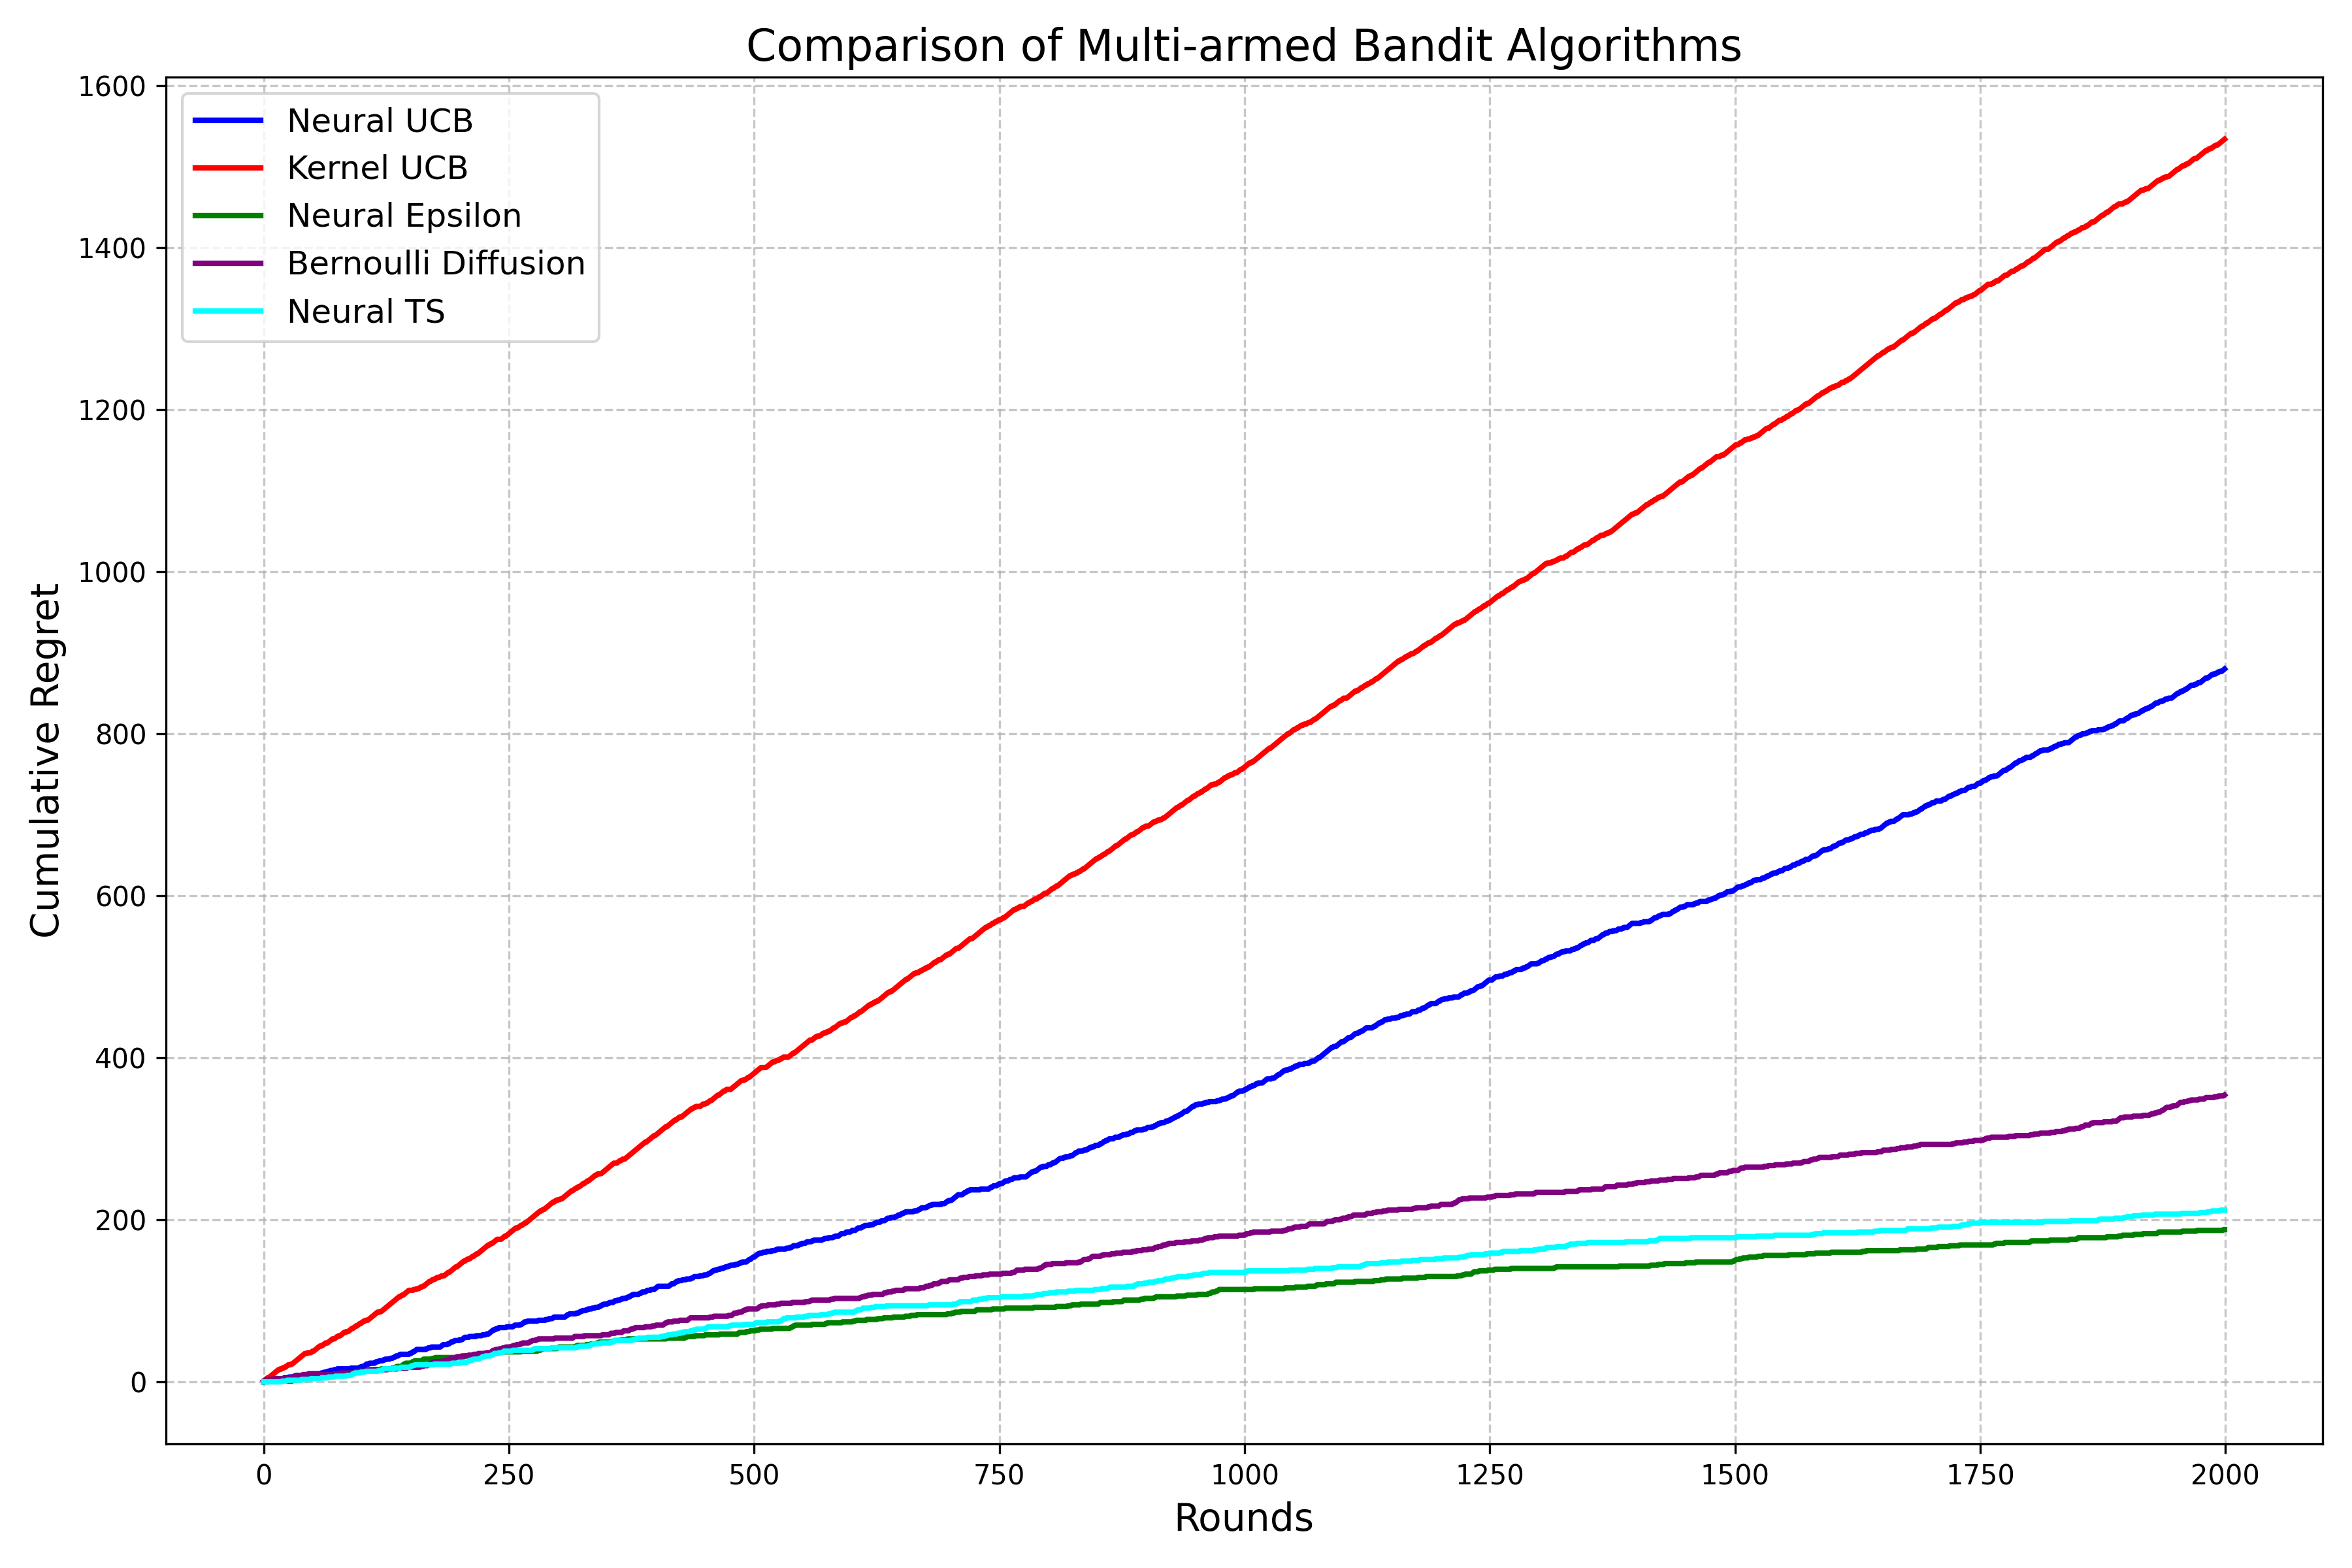
\includegraphics[width=\linewidth]{Img/context_compare.png}
\end{tikzfigure}